\documentclass[conference]{IEEEtran}
\IEEEoverridecommandlockouts

\usepackage{listings}
\usepackage{float}
\usepackage[spanish, es-tabla, es-nodecimaldot]{babel}
\usepackage{cite}
\usepackage{amsmath,amssymb,amsfonts}
\usepackage{algorithmic}
\usepackage{graphicx}
\usepackage{textcomp}
\usepackage{xcolor}
\lstset{basicstyle=\small\ttfamily,columns=fullflexible}

% preambulo:
%\usepackage[utf8]{inputenc}
% caracteres utf8 (tildes, enie) sin tener que usar comandos


%% NO AGREGAR PAQUETES ANTES DE ESTO, ES IMPORTANTE QUE BABEL ESTE PRIMERO

%%%%%%%%%%%%%%%%%%%%%%%%%%%%%%%%%
%% PAQUETES EXTRA %%%%%%%%%%%%%%%
%%%%%%%%%%%%%%%%%%%%%%%%%%%%%%%%%

\usepackage{subfiles}

\usepackage{cite}
\usepackage{amsmath,amssymb,amsfonts}
\usepackage{algorithmic}
\usepackage{textcomp}
\usepackage{xcolor}

\usepackage{steinmetz} % comando \phase{}
\usepackage{units} % permite usar nicefrac
\usepackage{graphicx} % importar imagenes
\usepackage{float} % posicion H para floats
\usepackage[colorinlistoftodos]{todonotes}


\usepackage[a4paper, total={6in, 8in}]{geometry} 
% margenes correctos en subarchivos

\setlength{\parindent}{10pt}			%cuanta sangria al principio de un parrafo
\usepackage{indentfirst}				%pone sangria al primer parrafo de una seccion

\def\BibTeX{{\rm B\kern-.05em{\sc i\kern-.025em b}\kern-.08em
    T\kern-.1667em\lower.7ex\hbox{E}\kern-.125emX}}


%%%%%%%%%%%%%%%%%%%%%%%%%%%%%%%%%%%%%%%%%%%%%%%%%%%%%%%%%%%
%% NO AGREGAR PAQUETES DESPUES DE ESTO, ES IMPORTANTE QUE HYPERREF ESTE ULTIMO
\usepackage[hidelinks]{hyperref} % hipervinculos sin cajitas rojas

\usepackage[spanish, es-tabla, es-nodecimaldot]{babel} 
% texto automatico en espaniol
% "tabla" en vez de "cuadro"
% no reemplaza puntos decimales por comas

\usepackage{listings}
\usepackage{float}
\lstset{basicstyle=\small\ttfamily,columns=fullflexible}



\def\BibTeX{{\rm B\kern-.05em{\sc i\kern-.025em b}\kern-.08em
    T\kern-.1667em\lower.7ex\hbox{E}\kern-.125emX}}
\begin{document}

\title{Retoque fotográfico mediante reconstrucciones geométricas heurísticas}
\author{\IEEEauthorblockN{Ariel Nowik, Joaquin Mestanza, Rocio Parra, Martina Máspero, Marcelo Regueira}
\IEEEauthorblockA{22.05 - Análisis de Señales y Sistemas Digitales - Grupo 1} \\
\textit{ITBA: Instituto tecnológico de Buenos Aires}\\
Ciudad de Buenos Aires, Argentina
}
\maketitle

\begin{abstract}
En este trabajo se estudiaron
 diversos métodos de retoque de imagenes para eliminar elementos no deseados presentes en diversas fuentes. Finalmente se procedió a realizar una implementación en función de las tecnicas analizadas seguida de un análisis de sus ventajas y desventajas.
\end{abstract}

\section{Introducción}
El problema elemental a resolver consiste en la eliminación de un objeto no deseado en una imagen.
Naturalmente no es posible "adivinar" lo que se encuentre por detrás, ya que requiere información adicional, la cual en principio no es accesible, solo se dispone de la imagen. Por lo tanto la idea es, de algun modo asimilar la zona de la imagen a reemplazar con el resto de la misma. En lo que continua de este trabajo describiremos con un mayor detalle diversos métodos para llevar a cabo este proceso.

\subsection{Descripción general del algoritmo}
El algoritmo trabajo en varias etapas. En cada iteración del algoritmo se ejecuta cada paso una vez. 
\begin{itemize}
	\item Cálculo del borde
	\item Selección del punto del borde a eliminar
	\item Selección de rectángulo correspondiente para el reemplazo
	
\end{itemize}

\begin{figure}[!ht]
\begin{centering}
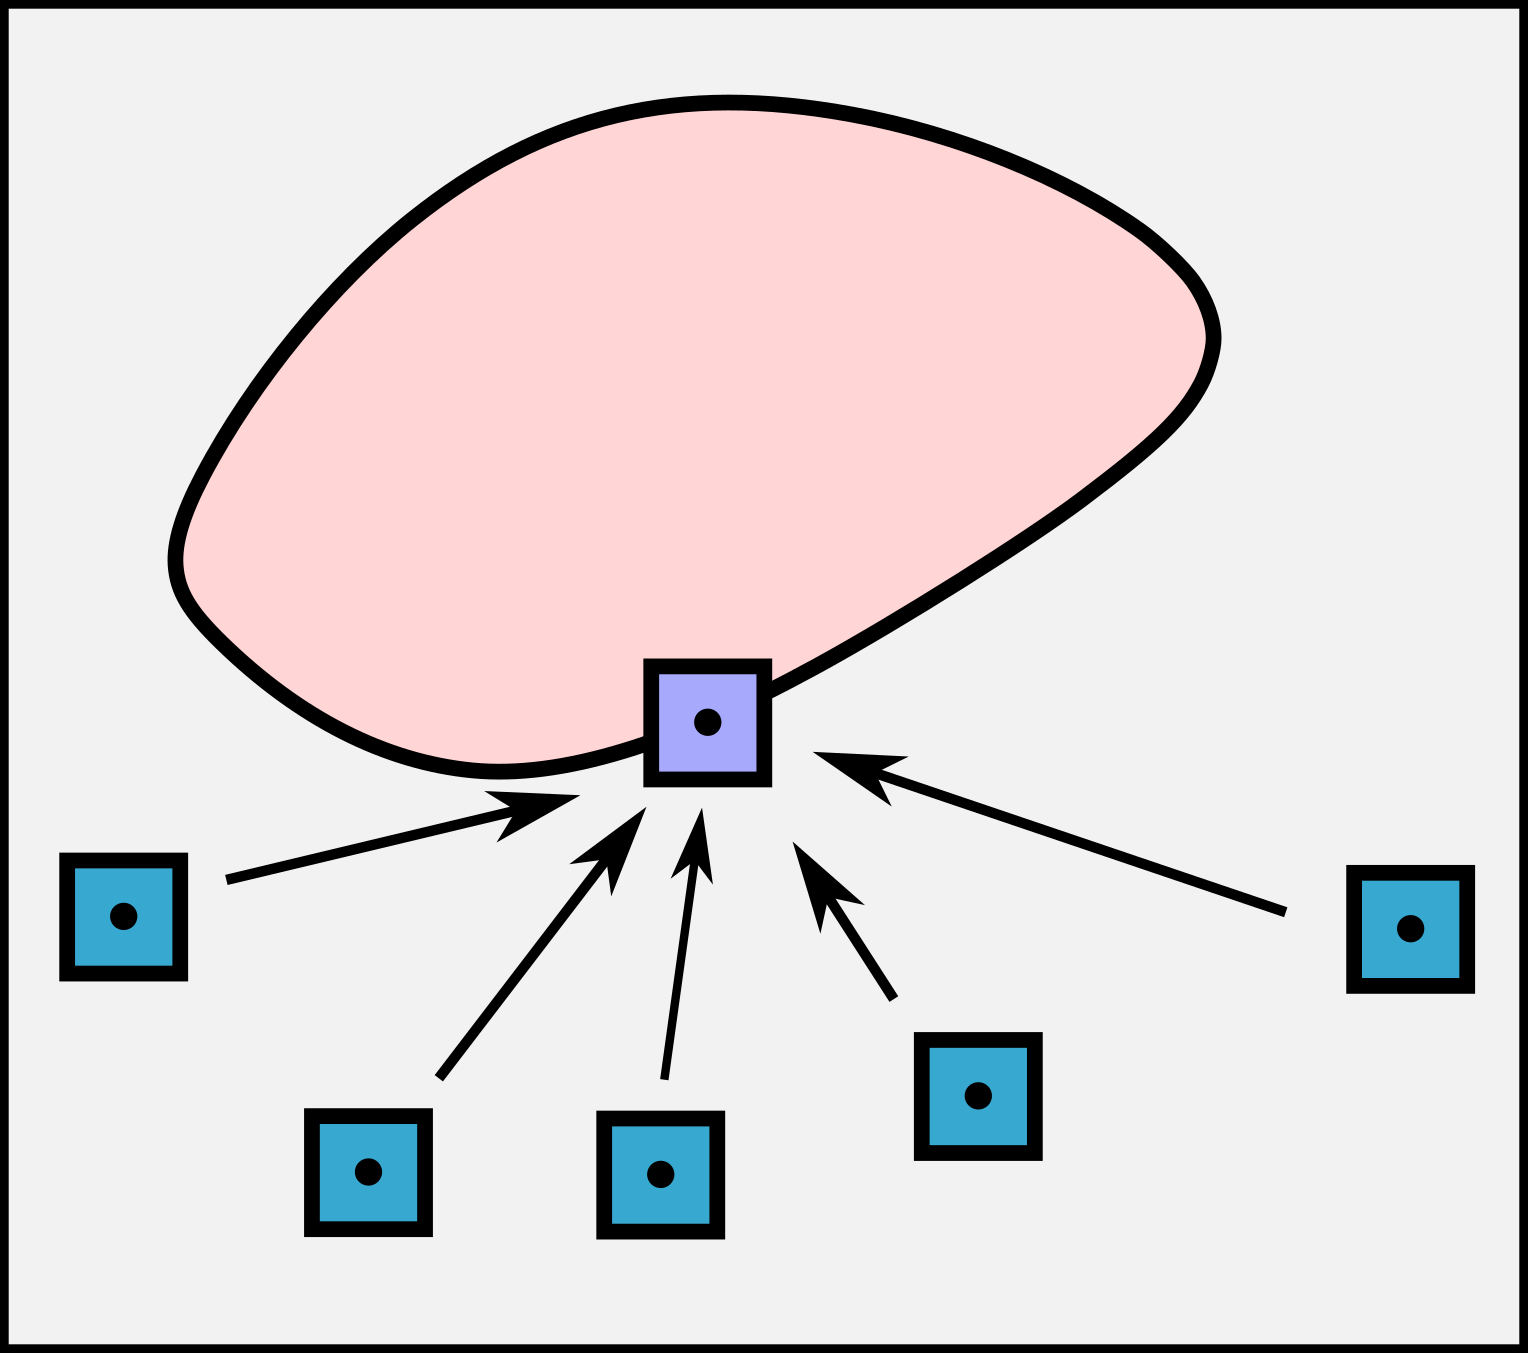
\includegraphics[scale=1]{descripcion.png}
\par\end{centering}
\caption{Descripción gráfica de una iteración del algoritmo}
\end{figure}

A medida que avanza el algoritmo se va disminuyendo el tamaño de la región a eliminar ya que se la asimila a los pixeles que estan por fuera. Cuando dicha región ya no existe se termina de correr el programa.

\subsection{Descripción de la zona a eliminar}
Es muy importante que el usuario que necesite retocar la imagen "indique" que región sea necesaria eliminar. En nuestro algoritmo decidimos que se ingrese como entrada una imagen de dos colores "blanco" y "negro" donde la zona negra sea aquella que se necesite borrar. En el desarrollo de el método muchas veces es necesario trabajr con el borde de esta región; se estudió entonces como utilizar la librería opencv que es muy conocida en el ambito de procesamiento de imagenes, la cual ofreció métodos optimizados para la detección de bordes de tanto regiones conexas, como regiones "multiplemente conexas"


\subsection{Cálculo de gradientes de imagen}
Para el funcionamiento del algoritmo fue necesario el cálculo de los gradientes de la imagen. Para ello se cálculo primero la imagen en una escala de grises y luego se aplicó el operador Sobel, el cual combinó tanto derivada como suavización gaussiana. 

\subsection{Determinación de prioridades}
En cada iteración se necesito calcular de todos los pixeles del borde aquellos con una mayor prioridad para ser asimilados. En los papers citados se muestran fundamentos por los cuales es más apropiado poderar por un lado el gradiente de la imagen y por el otro la confianza 
\begin{figure}[!ht]
\begin{centering}
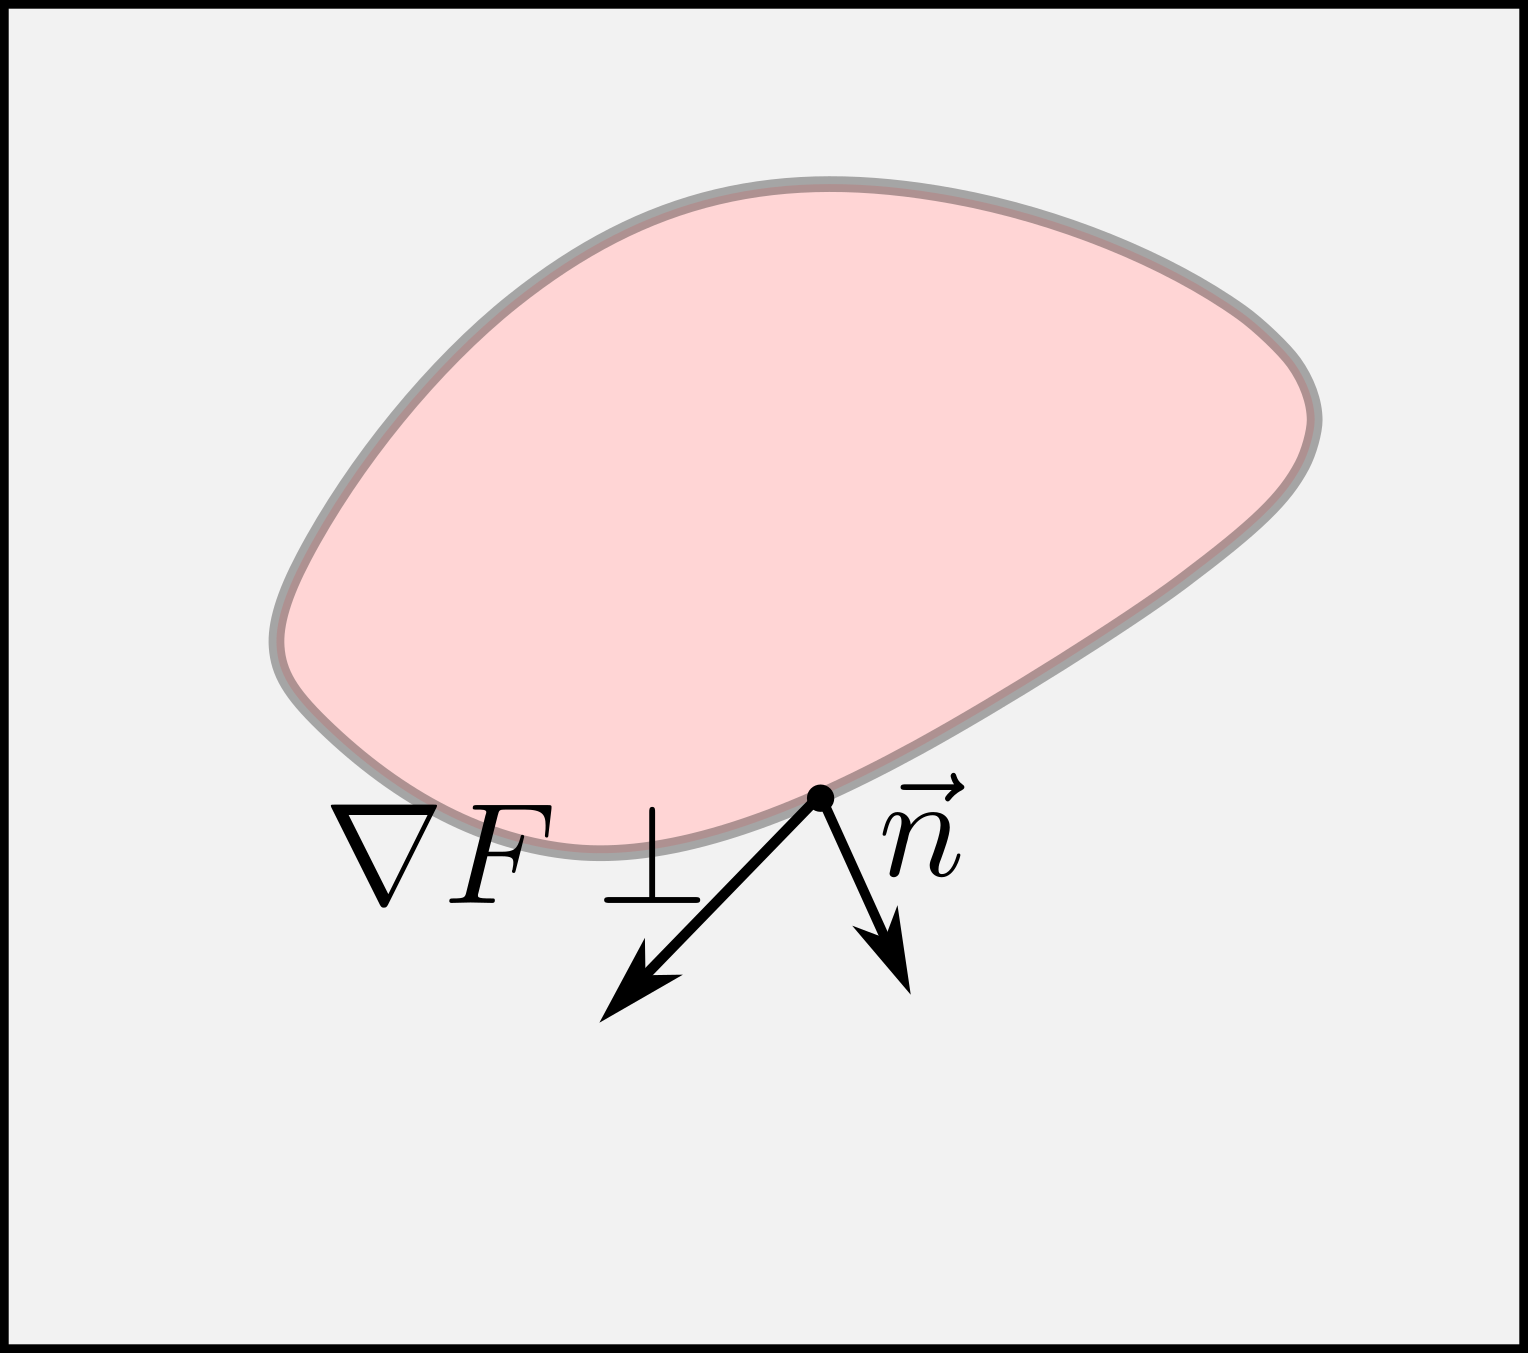
\includegraphics[scale=1]{normal_gradiente.png}
\par\end{centering}
\caption{Gradiente y normal}
\end{figure}
La formula que determina la prioridad esta dada por
\begin{equation}
P_i = C_i \nabla  F_i \perp \vec n_i
\end{equation}
Donde $\nabla F_i \perp$ es la perpendicular al gradiente de la imagen en el pixel $i$. Es el punto donde ocurre el cambio más suave en la intensidad del color de la imagen. El algoritmo realiza el producto escalar entre $\nabla F_i \perp \vec n_i$ lo cual consigue la componente normal del la perpendicular al gradiente, que nos indica que tan suave cambia la intensidad de la imagen en la dirección normal al borde de la región

\subsection{Determinación del rectángulo a reemplazar}
Para mejorar la eficiencia del algoritmo se decidió elegir rectángulos eficientes al rededor del pixel para asimilar el pixel de la imagen a la textura. Se comparó entre todos los candidatos utilizando la norma 2 comparando el cuadrado de la región a reemplazar y el candidato. A continuación se muestra la fórmula utilizada para el cálculo de de norma 2
\begin{equation}
\sum{(R_{1i}-R_{2i})^2+(G_{1i}-G_{2i})^2+(B_{1i}-B_{2i})^2}
\end{equation}
Se utilizó una distribución normal para elegir al azar los cantidatos 
\subsection{Parámetros, ventajas y desventajas}
Finalmente con el algoritmo implementado se probó variar diversos parárametros, entre ellos:
\begin{itemize}
	\item Tamaño de los cuadrados
	\item Region para buscar cuadrados
	\item Cantidad de muestros
\end{itemize}
Variando dichos parámetros en generar el "tradeoff" fue eficiencia vs una mejor calidad en el procesamiento de la imagen
\section{Resultados}
A continuación se mostrará una selección con los resultados del algoritmo
\subsection{Ejemplo 1}
Se procedió a probar el algoritmo con una moneda en un fondo de textura prácticamente unifirme
\begin{figure}[H]
\begin{centering}
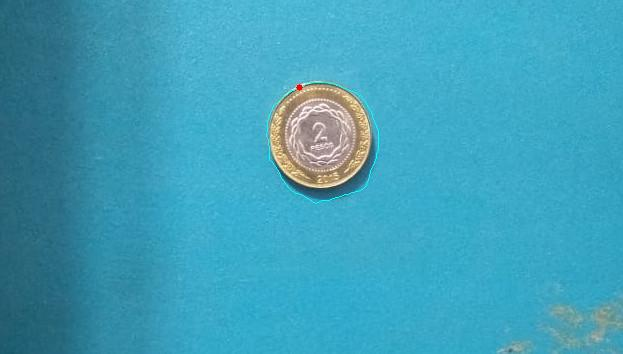
\includegraphics[scale=0.19]{moneda1.jpeg}
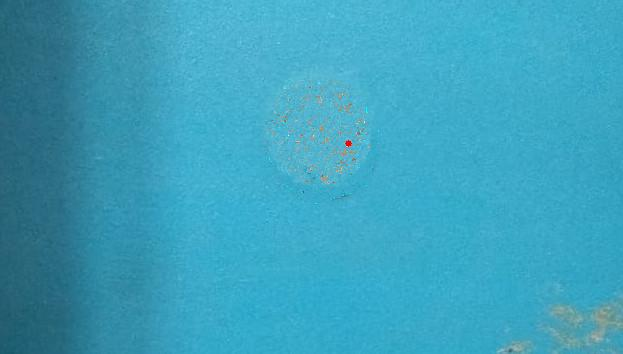
\includegraphics[scale=0.19]{moneda2.jpeg}
\par\end{centering}
\caption{Resultados - ejemplo 1}
\end{figure}
Si bien se notaron algunas impurezas dado que fue la primera versión del algoritmo, los resultados fueron satisfactorios
\subsection{Ejemplo 2}
Se probó el algoritmo esta vez con un fondo gris y unas piedritas de decoración
\begin{figure}[H]
\begin{centering}
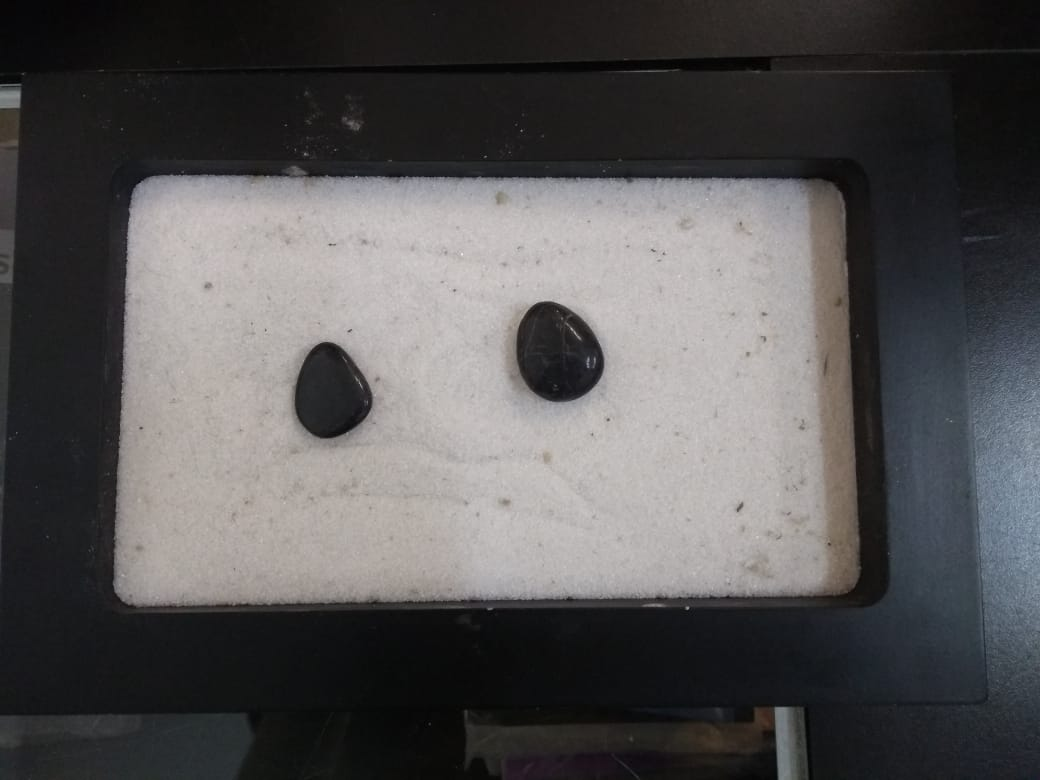
\includegraphics[scale=0.11]{imagen.jpeg}
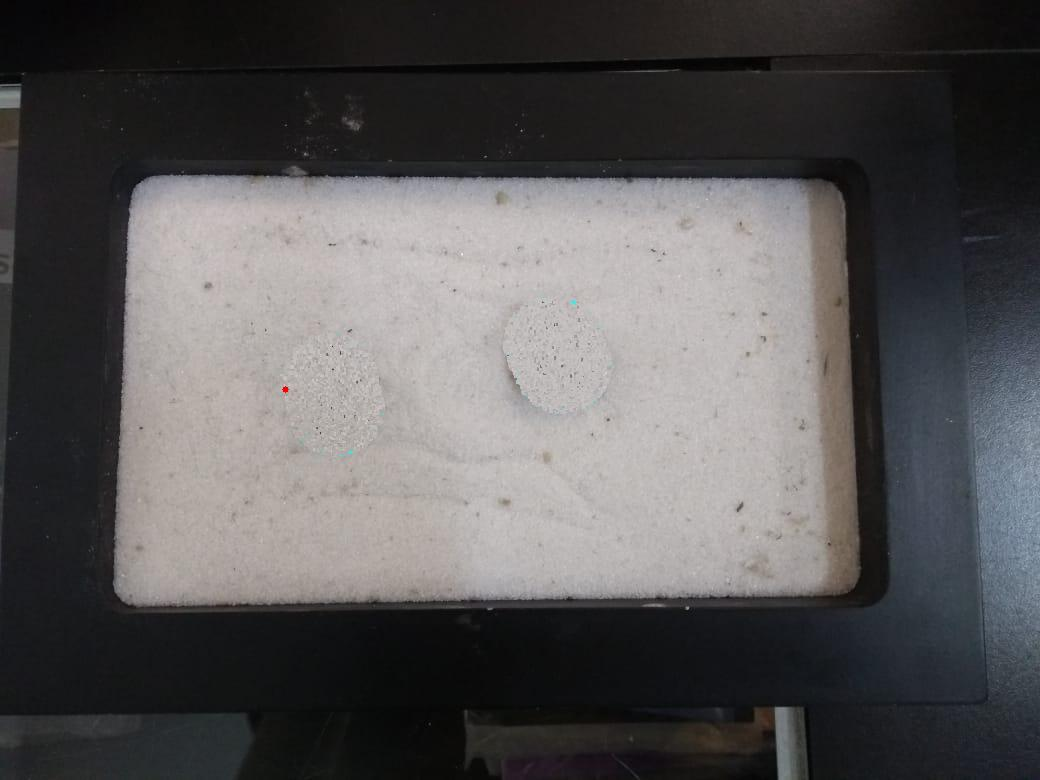
\includegraphics[scale=0.11]{imagen3320.jpeg}
\par\end{centering}
\caption{Resultados - ejemplo 2}
\end{figure}
Se obeservó que si bien se logró cubrir correctamente las areas a eliminar, la transcisión de colores no fue totalmente continua. Esto induce a que en un futuro se desarrolle algun procedimiento adicional que suavice dicha transición
\subsection{Ejemplo 3}
El tercer ejemplo fue corrido luego de convertir la distribución de la elección de cuadrados de lineal a gaussiana
\begin{figure}[H]
\begin{centering}
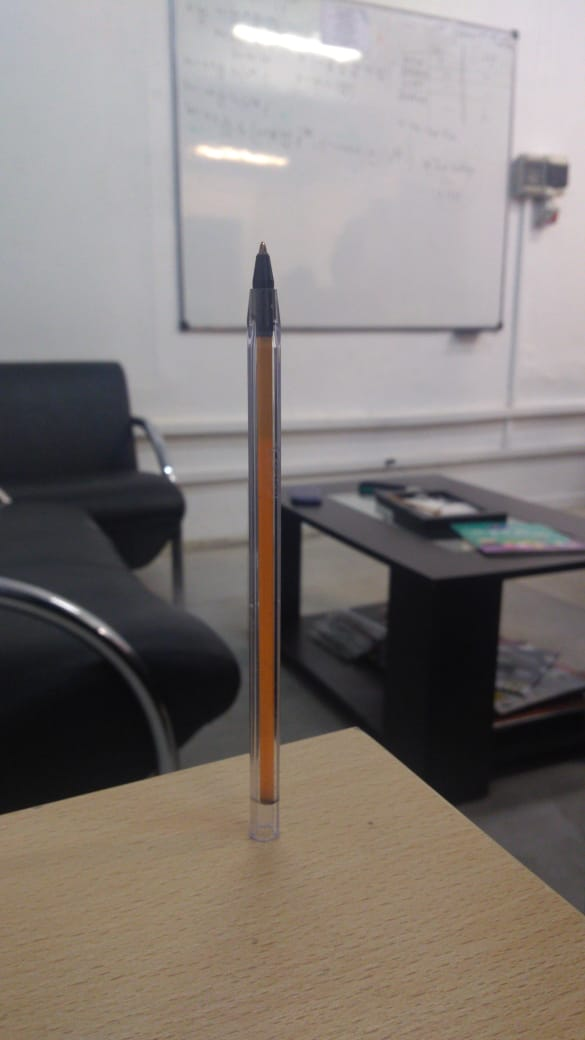
\includegraphics[scale=0.18]{imagen3.jpeg}
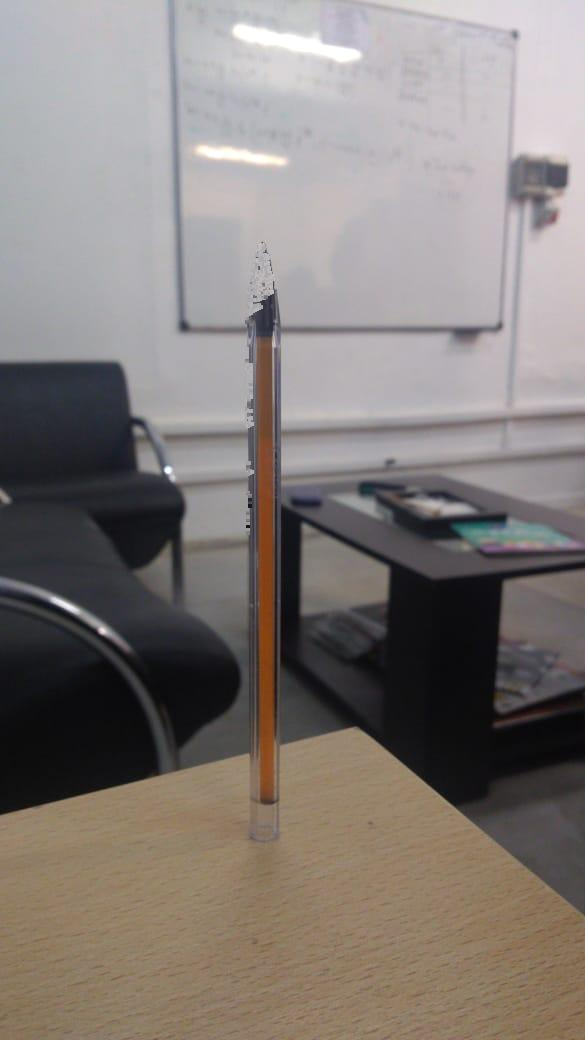
\includegraphics[scale=0.18]{imagen280.jpeg}
\par\end{centering}
\caption{Resultados - ejemplo 3}
\end{figure}
Se corrieron solo 280 iteraciónes del algoritmo pero se observaron resultados satisfactorios, el algoritmo tendió a absorber la lapicera.

\section{Código}

\lstinputlisting[linewidth=\columnwidth,breaklines=true]{main.py}

\begin{thebibliography}{00}
\bibitem{b1} A. Criminisi, P. Perez, and K. Toyama, “Region filling and object ´
removal by exemplar-based image inpainting,” IEEE T. Image Process.,
vol. 13, no. 9, pp. 1200–1212, Sep. 2004.

\bibitem{b2} Pierre Buyssens, Maxime Daisy, David Tschumperlé, Olivier Lézoray. Exemplar-based Inpainting:
Technical Review and new Heuristics for better Geometric Reconstructions. IEEE Transactions on
Image Processing, Institute of Electrical and Electronics Engineers, 2015, 24 (6), pp.1809 - 1824.
ff10.1109/TIP.2015.2411437ff. ffhal-01147620f
\end{thebibliography}
\end{document}
